\newgeometry{top=1cm, bottom=2cm}
\section{Lineare Differentialgleichungssysteme}
\begin{figure}[h!]
    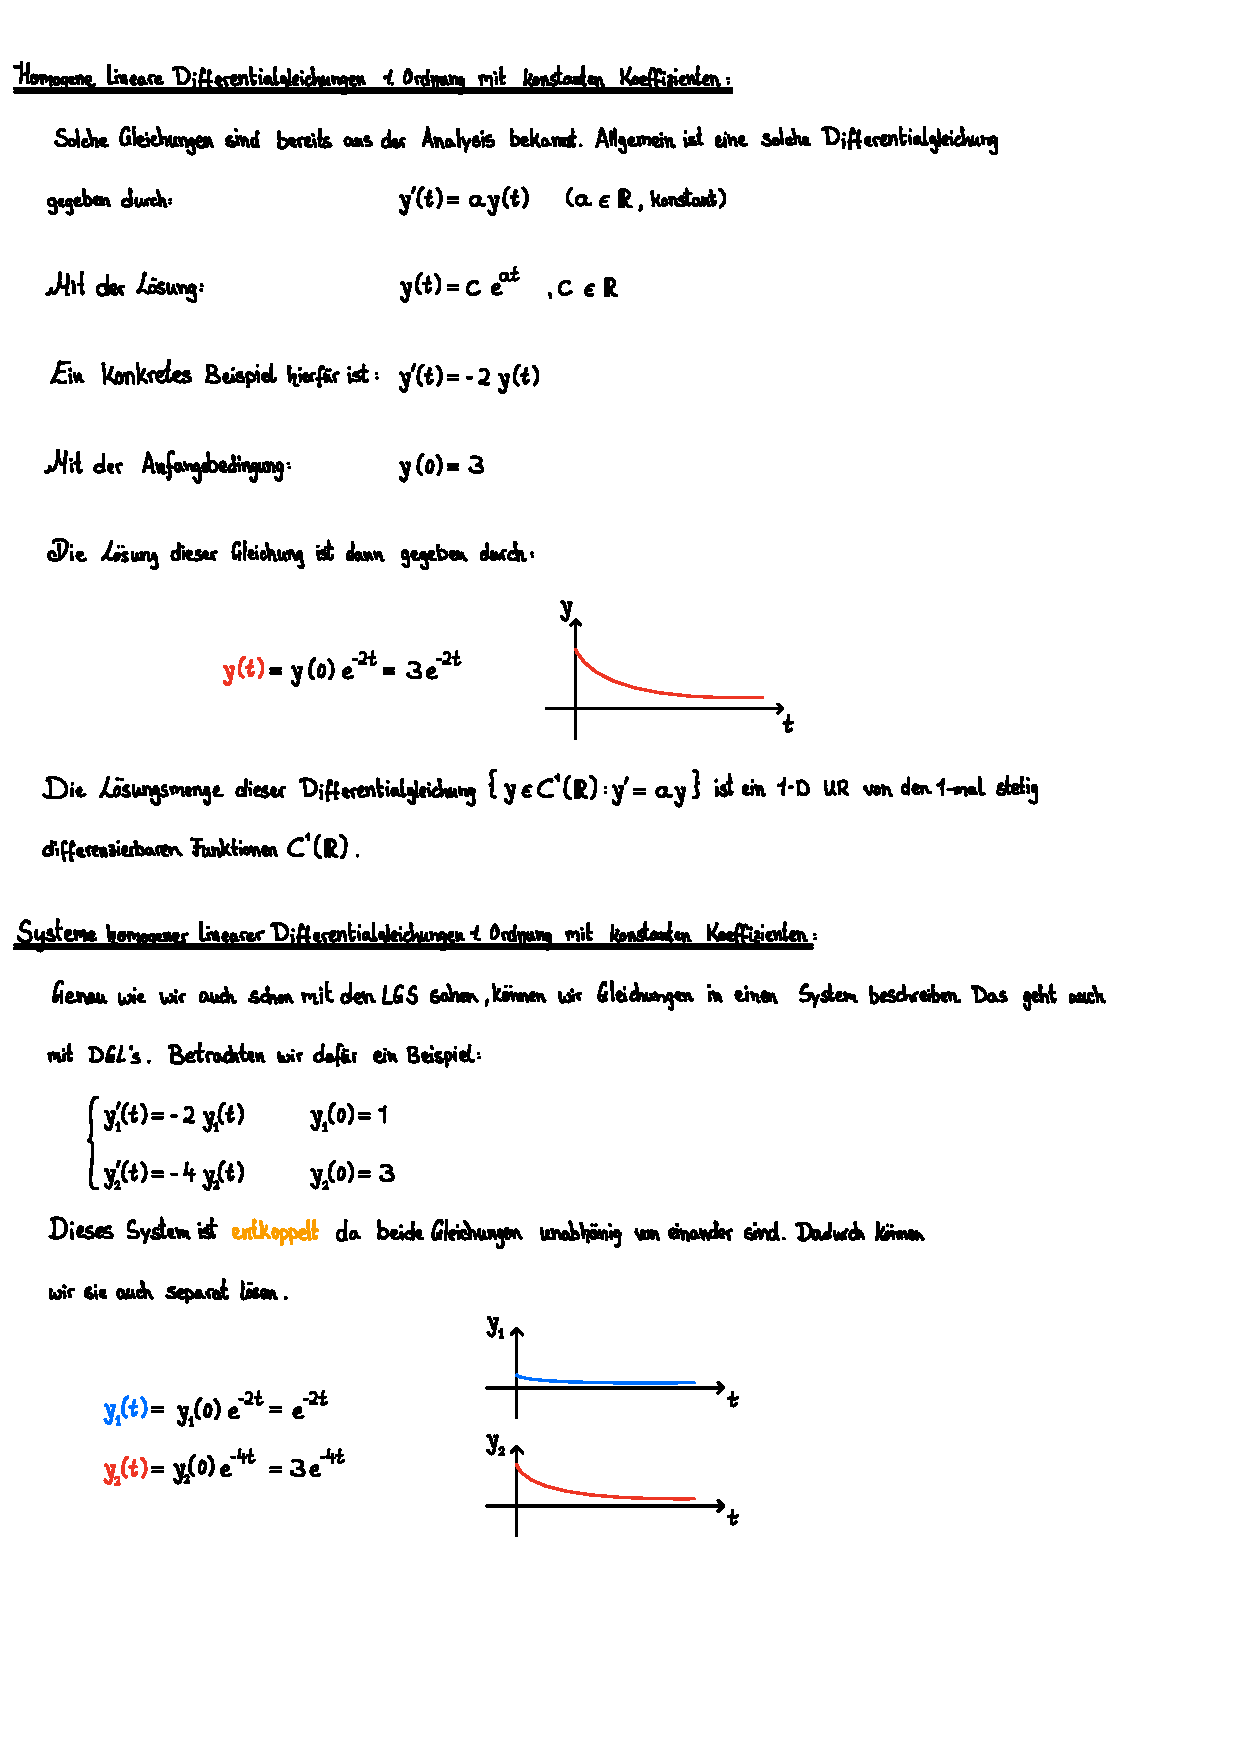
\includegraphics[page=1, scale=0.842]{pdf/08_Lineare_diff_systeme.pdf}
\end{figure}
\newpage
\includepdf[pages={2-}, 
            pagecommand={\thispagestyle{plain}}, 
            scale=0.95]{pdf/08_Lineare_diff_systeme.pdf}

\newgeometry{top=2.5cm, bottom=2cm}

\subsection{Beispielaufgaben}

\vspace{1cm}

\subsubsection{} %Zardini S. 137

Sei \[ A = \begin{pmatrix} 1 & 1 \\ 6 & 2 \\ \end{pmatrix}. \] Lösen Sie das Anfangswertproblem \[ y'=Ay \;, \; y(0)= \begin{pmatrix} 0 \\ 10 \\ \end{pmatrix} \]

\vspace{1\baselineskip}

\begin{solution}    

    \leftskip=2em

    \begin{equation*}
        \begin{vmatrix}
            1-\lambda & 1\\
            6 & 2-\lambda
        \end{vmatrix} = (1-\lambda)(2-\lambda) - 6 = \lambda^2 - 3\lambda - 4 = (\lambda-4)(\lambda+1) = 0
    \end{equation*}

    \begin{equation*}
        \lambda_1 = 4, \quad \lambda_2 = -1
    \end{equation*}

    \( E_4: \)

    \begin{equation*}
        \begin{gmatrix}[L]
            -3 & 1\\
            6 & -2
        \end{gmatrix} \hspace{-0.75em} \begin{gmatrix}[R]
            0\\
            0
        \end{gmatrix} \rightarrow \begin{gmatrix}[L]
            -3 & 1\\
            0 & 0
        \end{gmatrix} \hspace{-0.75em} \begin{gmatrix}[R]
            0\\
            0
        \end{gmatrix} \; \rightarrow \; \left\{ \begin{aligned}
            x_2 &= t \\
            x_1 &= \frac{t}{3}
            \end{aligned} 
        \right. \qquad E_4 = \text{span} \left\{ \begin{pmatrix} 1 \\ 3 \end{pmatrix} \right\}
    \end{equation*}

    \( E_{-1}: \)
    \begin{equation*}
        \begin{gmatrix}[L]
            2 & 1\\
            6 & 3
        \end{gmatrix} \hspace{-0.75em} \begin{gmatrix}[R]
            0\\
            0
        \end{gmatrix} \rightarrow \begin{gmatrix}[L]
            2 & 1\\
            0 & 0
        \end{gmatrix} \hspace{-0.75em} \begin{gmatrix}[R]
            0\\
            0
        \end{gmatrix} \; \rightarrow \; \left\{ \begin{aligned}
            x_2 &= t\\
            x_1 &= -\frac{t}{2}
            \end{aligned} 
        \right. \qquad E_{-1} = \text{span} \left\{ \begin{pmatrix} 1 \\ -2 \end{pmatrix} \right\}
    \end{equation*}

    Die allgemeine Lösung ist also

    \begin{equation*}
        y(t) = c_1 \begin{pmatrix} 1 \\ 3 \end{pmatrix} e^{4t} + c_2 \begin{pmatrix} 1 \\ -2 \end{pmatrix} e^{-t}
    \end{equation*}

    Nun fehlt noch die Anfangsbedingung

    \begin{equation*}
        y(0) = c_1 \begin{pmatrix} 1 \\ 3 \end{pmatrix} + c_2 \begin{pmatrix} 1 \\ -2 \end{pmatrix} = \begin{pmatrix} 0 \\ 10 \end{pmatrix} \rightarrow \; \begin{gmatrix}[L]
            1 & 1\\
            3 & -2
        \end{gmatrix} \hspace{-0.75em} \begin{gmatrix}[R]
            0\\
            10
        \end{gmatrix} \; \rightarrow \; c_1 = -c_2 = 2
    \end{equation*}

    Damit ist die Lösung des Anfangswertproblems

    \begin{equation*}
        y(t) = 2 \begin{pmatrix} 1 \\ 3 \end{pmatrix} e^{4t} - 2 \begin{pmatrix} 1 \\ -2 \end{pmatrix} e^{-t} = \begin{pmatrix} 2e^{4t} - 2e^{-t} \\ 6e^{4t} + 4e^{-t} \end{pmatrix}
    \end{equation*}

\end{solution}

\newpage

\subsubsection{} %Übung 11 (S17)

Gegeben sei die Differentialgleichung 2. Ordnung

\begin{equation}
    x''(t) = -8x(t) + 4x'(t)  
    \tag{$\dagger$}
\end{equation}

\begin{enumerate}[label=\alph*)]
    \item Verwandeln Sie (\( \dagger \)) in ein Differentialgleichungssystem 1. Ordnung. Welche Dimension hat der Lösungsraum dieses Systems?
    \item Geben Sie die allgemeine reelle Lösung der Differentialgleichung (\( \dagger \)) an.
    \item Bestimmen Sie die Lösung von (\( \dagger \)) zu den Bedingungen \( x(0) = 1, x(\frac{\pi}{4})=1 \).
\end{enumerate}

\vspace{1\baselineskip}

\begin{solution}    

    \vspace{1\baselineskip}

    \leftskip=2em

    \textbf{a)} Zuerst wandeln wir (\( \dagger \)) in ein System 1. Ordnung um. Die Substitution

    \begin{equation*}
        \begin{aligned}
            y_0 &:= x \\
            y_1 &:= x' \\
            y_2 &:= x''         
        \end{aligned} \qquad \longrightarrow \qquad
        \begin{aligned}
            y_1 = y_0' \\
            y_2 = y_1' 
        \end{aligned}
    \end{equation*}   

    führt zu dem Differentialgleichungssystem
    
    \begin{equation*}
        \left\{ \begin{aligned}
            y_0' &= y_1 \\
            y_1' &= -8y_0 + 4y_1
        \end{aligned} \right. \qquad \text{bzw.} \qquad
        \begin{pmatrix}
            y_0' \\
            y_1'
        \end{pmatrix} =
        \underbrace{\begin{pmatrix}
            0 & 1 \\
            -8 & 4
        \end{pmatrix}}_{A}
        \begin{pmatrix}
            y_0 \\
            y_1
        \end{pmatrix}.
    \end{equation*}

    \textbf{b)} Allgemeine \textbf{reelle} Lösung finden. 

    \begin{equation*}
        \text{det} \begin{pmatrix}
            -\lambda & 1 \\
            -8 & 4 - \lambda
        \end{pmatrix} = \lambda^2 - 4\lambda + 8 = 0 \quad \rightarrow \quad
        \lambda_{1,2} = 2 \pm 2i,
    \end{equation*}

    \begin{equation*}
        E_{2+2i} : \begin{gmatrix}[L]
            -2-2i & 1 \\
            -8 & 2-2i
        \end{gmatrix} \hspace{-0.75em}
        \begin{gmatrix}[R]
            0 \\ 0
            \rowops
            \add[\cdot\frac{-8}{2+2i}]{0}{1}
        \end{gmatrix} \rightarrow \quad
        \begin{gmatrix}[L]
            -2-2i & 1 \\
            0 & 0
        \end{gmatrix} \hspace{-0.75em}
        \begin{gmatrix}[R]
            0 \\ 0
        \end{gmatrix} \quad \left\{ \begin{aligned}
            y_0 &= \frac{s}{2+2i} \\[0.5em]
            y_1 &= s \in \mathbb{R} 
        \end{aligned} \right.
    \end{equation*}

    \vspace{1\baselineskip}

    \begin{equation*}
        \text{für} \ s = 4 \quad \left\{ \begin{aligned}
            y_0 &= \frac{4}{2+2i} \cdot \underbrace{\frac{2-2i}{2-2i}}_{=1} = \frac{4(2-2i)}{4+4} = 1-i \\
            y_1 &= 4 
        \end{aligned} \right.
    \end{equation*}

    \vspace{1\baselineskip}

    \begin{equation*}
        E_{2+2i} : \ \text{span} \left\{ \begin{pmatrix}
            1-i \\ 4
        \end{pmatrix} \right\} \ , \quad 
        E_{2-2i} : \ \text{span} \left\{ \begin{pmatrix}
            1+i \\ 4
        \end{pmatrix} \right\}.
    \end{equation*}

    Wodurch sich die folgende allgemeine Lösung des Systems ergibt

    \begin{equation*}
        y(t) = e^{(2+2i)t} \begin{pmatrix}
            1-i \\ 4
        \end{pmatrix} + e^{(2-2i)t} \begin{pmatrix}
            1+i \\ 4
        \end{pmatrix}.
    \end{equation*}

    Diese Lösung ist jedoch komplex. Normalerweise wollen wir aber eine reelle Lösung. Um eine reelle Lösung zu erhalten, benutzten wir die Eulersche Formel \( r e^{i \phi} = r \cos(\phi) + i \ r \sin(\phi) \). Um die Notation folgend zu vereinfachen betrachten, wir nur einen der beiden Eigenvektoren der Lösung (wenn man beide betrachtet kommt man auf das gleiche Ergebnis nur mit mehr Notation, am Ende findest du die Alternative mit beiden). 

    \begin{equation*}
        \begin{aligned}
            y(t) &= e^{(2+2i)t} \begin{pmatrix}
                1-i \\ 4
            \end{pmatrix} =
            e^{2t} e^{2it} \begin{pmatrix}
                1-i \\ 4
            \end{pmatrix} \\[0.5em]
            &= e^{2t} \left( \cos(2t) + i \sin(2t) \right) \begin{pmatrix}
                1-i \\ 4
            \end{pmatrix} \\[0.5em]
            &= e^{2t} \left\{ \begin{pmatrix}
                \cos(2t) + i \sin(2t) - i \cos(2t) - \sin(2t) \\
                4 \cos(2t) + 4i \sin(2t)
            \end{pmatrix} \right\} \\[0.5em]
            &= e^{2t} \left\{ \begin{pmatrix}
                \cos(2t) + \sin(2t) \\
                4 \cos(2t)
            \end{pmatrix} + i \begin{pmatrix}
                \sin(2t) - \cos(2t) \\
                4 \sin(2t)
            \end{pmatrix} \right\} 
        \end{aligned}
    \end{equation*}

    \vspace{0.5\baselineskip}

    Für den letzten Schritt benutzten wir ein Korollar aus der Vorlesung welches besagt, dass wenn \( y \) eine komplexe Lösung eines homogenen linearen Differentialgleichungssystems \( y'=Ay \) ist, so sind Re(\(y\)) und Im(\(y\)) ebenfalls Lösungen des Systems. Re(\(y\)) und Im(\(y\)) sind hier weiterhin linear unabhängig und bilden dadurch eine Basis des Lösungsraums von \( y \). So lässt sich eine allgemeine Lösung auch als Linearkombination von Re(\(y\)) und Im(\(y\)) schreiben

    \begin{equation*}
        y(t) = e^{2t} \left\{ a \begin{pmatrix}
            \cos(2t) + \sin(2t) \\
            4 \cos(2t)
        \end{pmatrix} + b \begin{pmatrix}
            \sin(2t) - \cos(2t) \\
            4 \sin(2t)
        \end{pmatrix} \right\}.
    \end{equation*}

    \vspace{0.5\baselineskip}

    Da wir eigentlich eine Lösung für \( (\dagger) \) suchen und durch die Substitution \( x = y_0 \) substituiert wurde, nehmen wir nur die erste Zeile des Vektors \( y(t) \). 

    \begin{equation*}
        \begin{aligned}
        x(t) = y_0(t) &= e^{2t} \left\{ a ( \cos(2t) + \sin(2t) ) + b ( \sin(2t) - \cos(2t) ) \right\} \\[0.5em]
        &= e^{2t} \left\{ (a-b) \cos(2t) + (a+b) \sin(2t) \right\} \\[0.5em]
        &= e^{2t} \left\{ c_1 \cos(2t) + c_2 \sin(2t) \right\}.
        \end{aligned}
    \end{equation*}

    \textbf{c)} Nun müssen wir die Anfangsbedingungen \( x(0) = 1 \) und \( x(\frac{\pi}{4})=1 \) in die allgemeine Lösung einsetzen.

    \begin{equation*}
        \begin{aligned}
            x(0) &= e^{2\cdot 0} \left\{ c_1 \cos(2\cdot 0) + c_2 \sin(2\cdot 0) \right\} = 1 \rightarrow c_1 = 1 \\[0.5em]
            x\left( \frac{\pi}{4} \right) &= e^{2\cdot \frac{\pi}{4}} \left\{ c_1 \cos\left( 2\cdot \frac{\pi}{4} \right) + c_2 \sin\left( 2\cdot \frac{\pi}{4} \right) \right\} = 1 \rightarrow c_2 = e^{-\frac{\pi}{2}}
        \end{aligned}
    \end{equation*}

    Damit ergibt sich die Lösung des Anfangswertproblems
    \begin{equation*}
        x(t) = e^{2t} \left\{ \cos(2t) + e^{-\frac{\pi}{2}} \sin(2t) \right\}.
    \end{equation*}

    \vspace{1\baselineskip}

    \textbf{Alternative Lösung mit beiden Eigenvektoren:}

    Anstatt nur einen der beiden Eigenvektoren zu benutzen, können wir auch beide benutzen. Das Resultat ist das gleiche, jedoch mit mehr Notationsaufwand.

    \begin{equation*}
        \begin{aligned}
            y(t) &= c_3 \cdot e^{(2+2i)t} \begin{pmatrix}
                1-i \\ 4
            \end{pmatrix} + c_4  \cdot e^{(2-2i)t} \begin{pmatrix}
                1+i \\ 4
            \end{pmatrix} \\[0.5em] 
            &= e^{2t} \left\{
                c_3 \left( 
                    \cos(2t) + i \sin(2t) \right) \begin{pmatrix}
                        1-i \\ 4
                    \end{pmatrix} + c_4  \left( 
                    \cos(2t) - i \sin(2t) \right) \begin{pmatrix}
                        1+i \\ 4
                    \end{pmatrix}
            \right\} \\[0.5em]
            &= e^{2t} \left( \text{\scriptsize $ \begin{matrix}
                c_3 \cos(2t) + c_3 i \sin(2t) - c_3 i \cos(2t) - c_3 \sin(2t) + c_4  \cos(2t) - c_4  i \sin(2t) + c_4  i \cos(2t) - c_4  \sin(2t) \\[0.5em]
                4 c_3 \cos(2t) + 4 c_3 i \sin(2t) + 4 c_4  \cos(2t) - 4 c_4  i \sin(2t)
            \end{matrix}$} \right) \\[0.5em]
            &= e^{2t} \left( \text{\scriptsize $ \begin{matrix}
                ( c_3 + c_4  ) \cos(2t) + ( c_3 - c_4  ) i \sin(2t) - ( c_3 - c_4  ) i \cos(2t) + ( c_3 + c_4  ) \sin(2t) \\
                4 ( c_3 + c_4  ) \cos(2t) + 4 ( c_3 - c_4  ) i \sin(2t)
            \end{matrix}$} \right) \\[0.5em]
            &= e^{2t} \left\{ \left( \text{\scriptsize $ \begin{gmatrix}[n]
                ( c_3 + c_4  ) \cos(2t) + ( c_3 + c_4  ) \sin(2t) \\
                4 ( c_3 + c_4  ) \cos(2t)
            \end{gmatrix} + i \begin{gmatrix}[m]   
                ( c_3 - c_4  ) \sin(2t) - ( c_3 - c_4  ) \cos(2t) \\
                4 ( c_3 - c_4  ) \sin(2t)
            \end{gmatrix}$} \right) \right\} \\[0.5em]
            &= e^{2t} \left\{ a \begin{pmatrix}
                \cos(2t) + \sin(2t) \\
                4 \cos(2t)
            \end{pmatrix} + i \ b \begin{pmatrix}
                \sin(2t) - \cos(2t) \\
                4 \sin(2t)
            \end{pmatrix} \right\} 
        \end{aligned}
    \end{equation*}

    womit wir schliesslich durch dieselbe Argumentation von oben die Lösung für \((\dagger)\) finden

    \begin{equation*}
        \begin{aligned}
        x(t) = y_0(t) &= e^{2t} \left\{ a ( \cos(2t) + \sin(2t) ) + b ( \sin(2t) - \cos(2t) ) \right\} \\[0.5em]
        &= e^{2t} \left\{ (a-b) \cos(2t) + (a+b) \sin(2t) \right\} \\[0.5em]
        &= e^{2t} \left\{ c_1 \cos(2t) + c_2 \sin(2t) \right\}.
        \end{aligned}
    \end{equation*}

\end{solution}

\newpage

\subsubsection{} %Zardini S. 154

Gegeben sei das Differentialgleichungssystem 2. Ordnung

\begin{equation*}
    \begin{aligned}
    y''(t) &= -2y(t) + z(t)\\
    z'(t) &= -6y(t) + 3z(t)
    \end{aligned}
\end{equation*}

\begin{enumerate}[label=\alph*)]
    \item Verwandeln Sie das Differentialgleichungssystem in ein System 1. Ordnung. 
    \item Geben Sie die allgemeine Lösung des in a) gefundenen Systems an.
\end{enumerate} 

\vspace{1\baselineskip}

\begin{solution}    

    \vspace{1\baselineskip}

    \leftskip=2em

    \textbf{a)} Substitution
    \begin{equation*}
        \begin{aligned}
            y' &:= x \\
            y'' &:= x' 
        \end{aligned} \quad \rightarrow \quad
        \begin{aligned}
            x' &= -2y + z \\
            y' &= x \\
            z' &= -6y + 3z
        \end{aligned} \quad \rightarrow \quad
        \begin{pmatrix}
            x' \\
            y' \\
            z'
        \end{pmatrix} =
        \begin{pmatrix}
            0 & -2 & 1 \\
            1 & 0 & 0 \\
            0 & -6 & 3
        \end{pmatrix}
        \begin{pmatrix}
            x \\
            y \\
            z
        \end{pmatrix}.
    \end{equation*}

    \textbf{b)} Allgemeine Lösung finden

    \vspace{1\baselineskip}

    Eigenwerte und Eigenvektoren ergeben:

    \begin{equation*}
        \lambda_1 = 0, \ \lambda_2 = 1, \ \lambda_3 = 2  
    \end{equation*}

    \begin{equation*}
        v_1 = \begin{pmatrix} 0 \\ 1 \\ 2 \end{pmatrix}, \ v_2 = \begin{pmatrix} 1 \\ 1 \\ 3 \end{pmatrix}, \ v_3 = \begin{pmatrix} 2 \\ 1 \\ 6 \end{pmatrix}.
    \end{equation*}

    \vspace{1\baselineskip}

    \begin{equation*}
        D = \begin{pmatrix}
            0 & 0 & 0 \\
            0 & 1 & 0 \\
            0 & 0 & 2
        \end{pmatrix}, \quad
        T = \begin{pmatrix}
            0 & 1 & 2 \\
            1 & 1 & 1 \\
            2 & 3 & 6
        \end{pmatrix}
    \end{equation*}

    \vspace{1\baselineskip}

    Die Allgemeine Lösung des Systems ist also

    \begin{equation*}
        \begin{pmatrix}
            x \\
            y \\
            z
        \end{pmatrix} = c_1 \begin{pmatrix} 0 \\ 1 \\ 2 \end{pmatrix} + c_2 e^{t} \begin{pmatrix} 1 \\ 1 \\ 3 \end{pmatrix} + c_3 e^{2t} \begin{pmatrix} 2 \\ 1 \\ 6 \end{pmatrix}
    \end{equation*}

\end{solution}